 \section{Rezultate}
 
Rezultatele au fost generate, în sistemul de operare Linux, atât cu planificatorul Fast-Downward, cât și cu planificatorul Fast-Forward, în funcție de tipul problemei.

 
 
 \subsection{Problema fară aplicabilitate în lumea reală}
 \textbf{Comenzi și rezultate:}
 
Pentru a testa domeniul și cele două tipuri de problemă, ne-am folosit de planner-ul Fast-Downward și de următoarele comenzi:
\bigskip

./fast-downward.py domain\_reteta\_heuristics.pddl problem1\_reteta\_heuristics.pddl 

./fast-downward.py domain\_reteta\_heuristics.pddl problem2\_reteta\_heuristics.pddl 
\bigskip
Ieșirea generată se află în fișierele output1.sas și output2.sas. Datorită lungimii lor, nu vor fi afișate aici, dar se pot observa pașii făcuți pentru atingerea scopului.
\bigskip

De asemenea, ne-am folosit de capabilitățile de search ale acestui planner, prin utilizarea următoarelor euristici și comenzi:

\newline

 \begin{itemize}
    \setlength\itemsep{0em}
    \item Căutare prin A*:
    \newline
      \newline
    ./fast-downward.py domain\_reteta\_heuristics.pddl problem1\_reteta\_heuristics.pddl --heuristic "h=ff()" --search "astar(h)"
    
  
  \newline
    ./fast-downward.py domain\_reteta\_heuristics.pddl problem2\_reteta\_heuristics.pddl --heuristic "h=ff()" --search "astar(h)"
      \newline
      \newline
      Mai jos este ieșirea în urma utilizării euristicii pe problema cu prăjitura. Se poate observa că A* a ales produsele de cea mai bună calitate (cele cu numărul cel mai mic), și a obținut un cost al planului de 10, care e soluția optimă. 
      \newline
        \inputminted[linenos]{C}{cod/rez_problem_heuristic_astar.txt}
       \newline
      \newline
      La utilizarea euristicii pe problema cu pizza, se poate de asemenea observa că A* a ales produsele de cea mai bună calitate (cele cu numărul cel mai mic), și a obținut un cost al planului de 5. 
      \newline
        \inputminted[linenos]{C}{cod/rez_problem2_heuristic_astar.txt}   
        \newline
        \newline
    \item Căutare prin Greedy (Eager):
     \newline
      \newline
      ./fast-downward.py domain\_reteta\_heuristics.pddl problem1\_reteta\_heuristics.pddl --heuristic "h=ff()" --search "eager(single(h))"
       
  
  \newline
./fast-downward.py domain\_reteta\_heuristics.pddl problem2\_reteta\_heuristics.pddl --heuristic "h=ff()" --search "eager(single(h))"
    \newline
      \newline
    Mai jos este ieșirea în urma utilizării euristicii pe problema cu prăjitura. Se poate observa că, fiind o strategie greedy, a ales prima calitate pe care a întâlnit-o de fiecare dată și a obținut un cost al planului de 19, care nu e soluția optimă. 
      \newline
        \inputminted[linenos]{C}{cod/rez_problem_heuristic_eager_greedy.txt}
       \newline
      \newline
       La utilizarea euristicii pe problema cu pizza, se poate de asemenea observa că Greedy a ales calitatea primelor ingrediente pe care le-a întâlnit, și a obținut un cost al planului de 5. În acest caz, prin coincidență, costul primele ingrediente au fost defapt cele care au avut calitatea cea mai bună, deci a fost generat un plan pentru costul optim.
      \newline
        \inputminted[linenos]{C}{cod/rez_problem2_heuristic_eager_greedy.txt}    
    \item Căutare prin Greedy (Lazy):
    \newline
      \newline
    ./fast-downward.py domain\_reteta\_heuristics.pddl problem1\_reteta\_heuristics.pddl --heuristic "h=ff()" --search "lazy(single(h))"

    
  
  \newline
   ./fast-downward.py domain\_reteta\_heuristics.pddl problem2\_reteta\_heuristics.pddl --heuristic "h=ff()" --lazy(single(h))"
      \newline
      \newline
     Mai jos este ieșirea în urma utilizării euristicii pe problema cu prăjitura. Se poate observa că, fiind o strategie greedy, a ales prima calitate pe care a întâlnit-o de fiecare dată și a obținut un cost al planului de 19, care nu e soluția optimă. Diferența dintre această strategie și strategia Greedy (eager) este ordinea de cumpărare a ingredientelor. 
     \newline
        \inputminted[linenos]{C}{cod/rez_problem_heuristic_lazy_greedy.txt}
       \newline
      \newline
        La utilizarea euristicii pe problema cu pizza, se poate de asemenea observa că Greedy a ales calitatea primelor ingrediente pe care le-a întâlnit, și a obținut un cost al planului de 5. În acest caz, prin coincidență, costul primele ingrediente au fost defapt cele care au avut calitatea cea mai bună, deci a fost generat un plan pentru costul optim.
      \newline
        \inputminted[linenos]{C}{cod/rez_problem2_heuristic_lazy_greedy.txt}   

\end{itemize}

\subsection{Problema cu în lumea reală}
 \textbf{Comenzi și rezultate:}

\newline
  Am folosit planner-ul Fast-Forward pentru generarea rezultatelor pentru domeniul și cele două tipuri de probleme. Comenzile sunt următoarele:
  \newline
    \newline
  ./Contingent-FF -o domain\_reteta\_contingent.pddl -f problem\_reteta\_contingent.pddl
    \newline
./Contingent-FF -o domain\_reteta\_contingent.pddl -f problem2\_reteta\_contingent.pddl
  \newline
    \newline
    Pentru problema cu prajitura, rezultatul este următorul:
    \newline
        \inputminted[linenos]{C}{cod/rez_problem_contingent.txt}   
        
    \newline 
    \newline
    Se poate observa arborele ce se obține din acțiunile disponibile. Datorită predicatelor unknown stricat care sunt observate de acțiunea sense\_stricat, se creează ramuri, iar arborele ajunge să aibă înălțimea 17. Numărul total de acțiuni până la atingerea scopului este 65.
    \newline
    \newline
    Pentru problema cu pizza, rezultatul este următorul:
    \newline
        \inputminted[linenos]{C}{cod/rez_problem2_contingent.txt}   
        
    \newline 
    \newline
    Se poate observa ce se obține din acțiunile dinsponibile. Arborele ajunge să aibă înălțimea 15, iar numărul total de acțiuni până la atingerea scopului este 34. Pentru a vizualiza mai bine acest rezultat, am ales să îl reprezentăm grafic sub formă de arbore:
     \newline 
    \newline
    \begin{figure}[htb]
  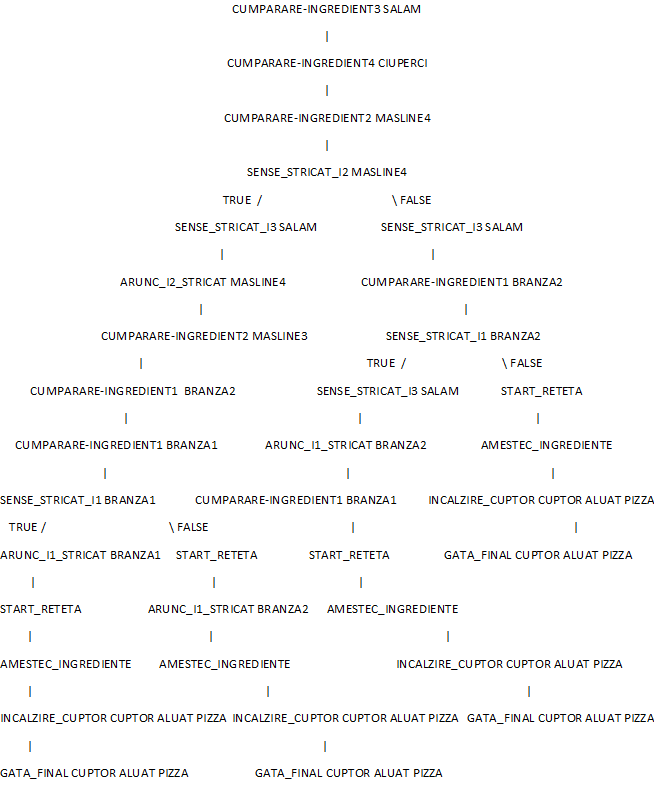
\includegraphics[width=\linewidth]{diagrama.png}
 \caption{Arborele generat de rezultatul problemei 2.}
  \label{fig:boat1}
  \end{figure}